\chapter{Plasma Control Systems}

\section{Overview of control systems}
The control of  plasma position, shape and current among other parameters is one of the crucial engineering problems for present and future magnetic confinement devices. The Plasma Control Systems (PCS) lead with the overall control of  fusion devices being responsible also for the  plasma configuration and scenarios algorithms \cite[Chapter~8]{PCS_2018}. Currently different PCS's are use in the tokamaks around the world. In this chapter the "DIII-D-like" PCS, the Syst\'eme de Contr\^ole Distribu\'e (SCD) and the Multi-threaded Application Real-Time executor (MARTe) will be approach, this last one being of special interest due to its extensive utilization in this work, likewise this chapter presents an overview of the equilibrium and control algorithms used for the reconstruction of plasma parameters and the controllers use for position,shape and plasma current among other parameters.

\subsection{DIII-D Plasma Control System}  

The DIII-D-like PCS is use in various fusion research facilities such as EAST(China), K-STAR (South Korea) and MAST (UK). Early documentation regarding the PCS in DIII-D\footnote{DIII-D is a D-shape tokamak operated by General Atomics in San Diego, California. } reefers to digitalization of analog signals transmitted to a high speed processor executing a shape control algorithm and then writing the result to a digital to analog converter for driving the controlled systems . The real-time computer used allowed to performed operations with vectors and matrices required for the plasma shape control algorithm \cite{DIIDcontrol}. Figure ~\ref{DIII1991} shows the block diagram of the DIII-D PCS 30 years ago.
\smallskip

\begin{figure}[htbp]
	\centering
	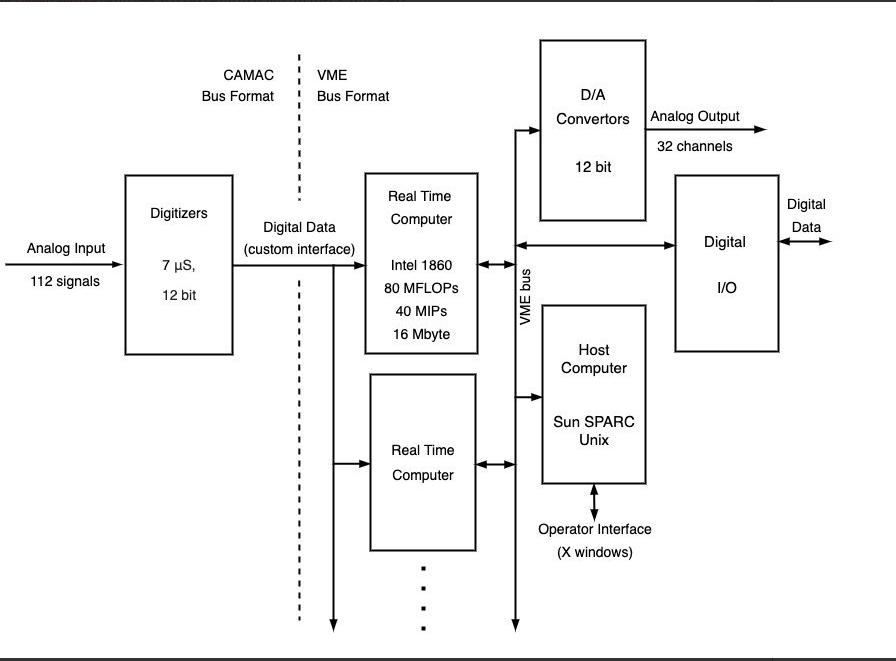
\includegraphics[width=0.65\textwidth]{Chp2/DIIDPCS_old.png}
	\caption{\label{DIII1991} DIII-D digital PCS in 1991 ~\cite{DIIDcontrol}.  }
\end{figure}

In recent years the DIII-D PCS had extensive software and hardware upgrades. The PCS actual software consists of an infrastructure library core which provides all the routines that are necessary for implementing a basic and generic control system. The current  PCS hardware configuration uses a collection of  Intel Linux based multi-processor computers running in parallel to perform the real-time analysis and feedback control ~\cite{DIIID2013}. New digitizers have been added to the real-time network to increase the number of signals acquired an to control hardware on real-time, several real-time control algorithms were added and real-time data was added to external entities such as web server.~\cite{DIIIDnew}. In the current version of the PCS, a Myricom\footnote{Myricom networks also called Myrnet are high speed networking systems used to interconnect machines to form computer clusters. } network has been replaced with a 40 Gb/sec InfiniBand\footnote{Is a network architecture from Mellanox designed to support I/O connectivity  and  reliability, availability, and serviceability Internet requirements ~\cite{MellanoxTechnologies2003}.  } network based on the Mellanox Connect-X 3\footnote{The Connect-X from the Mellanox company are Ethernet network interface cards with PCI Express.} hardware set. Figure ~\ref{DIIInew} shows the currently overall networking diagram of DIII-D PCS .


\begin{figure}[htbp]
	\centering
	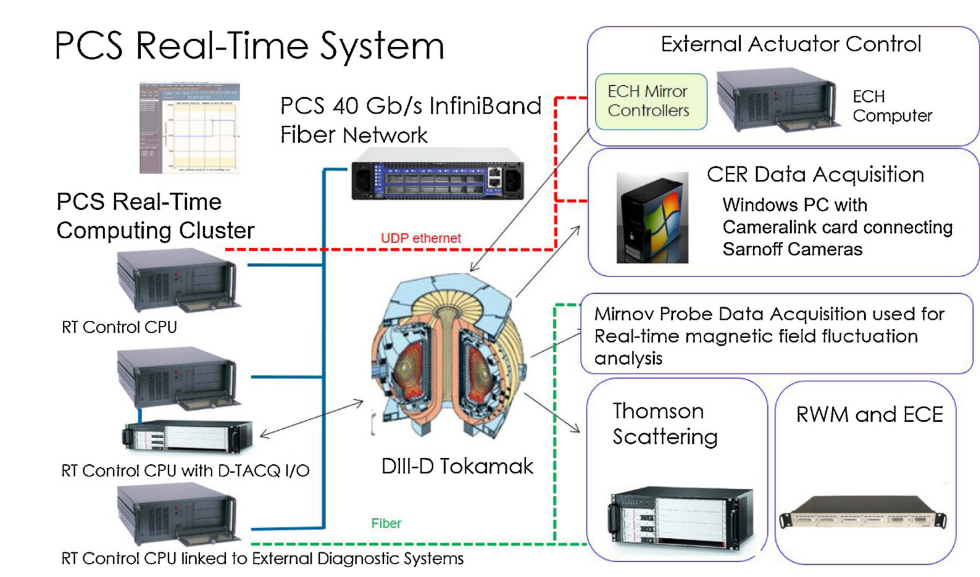
\includegraphics[width=0.65\textwidth]{Chp2/DIIIDPCSnew.PNG}
	\caption{\label{DIIInew} Actual DIII-D PCS real-time systems ~\cite{DIIIDnew}.  }
\end{figure}


\subsection{Syst\'eme de Contr\^ole Distribu\'e}

The TCV\footnote{The Tokamak \'a configuration variable (TCV) is  a medium size tokamak localized in Laussane,Switzerland. It is characterized by a highly elongated, rectangular vacuum vessel.} distributed control system uses a modular network of real time PC nodes liken by a real time network to provide feedback control over all of the actuator systems. Each node consists of a Linux PC either embedded on a Compact-PCI module or as a desktop computer with Intel CPU. A fiber optic ring network links the reflective memory (RFM) network cards in each node  \cite{TCVcntrl}.  The design of the diagnostic signal processing and control algorithms is performed in Matlab-Simulink software.  During the real-time execution  C/C++  code is generated from the Simulink and compiled  into a Linux shared library and distributed to target nodes  providing the input/output interface to the control algorithm code  ~\cite{TCVcntrl1}. Figure ~\ref{TCVcontrol} depicts the TCV SCD layout with the connectivity to diagnostics and actuators.


\begin{figure}[htbp]
	\centering
	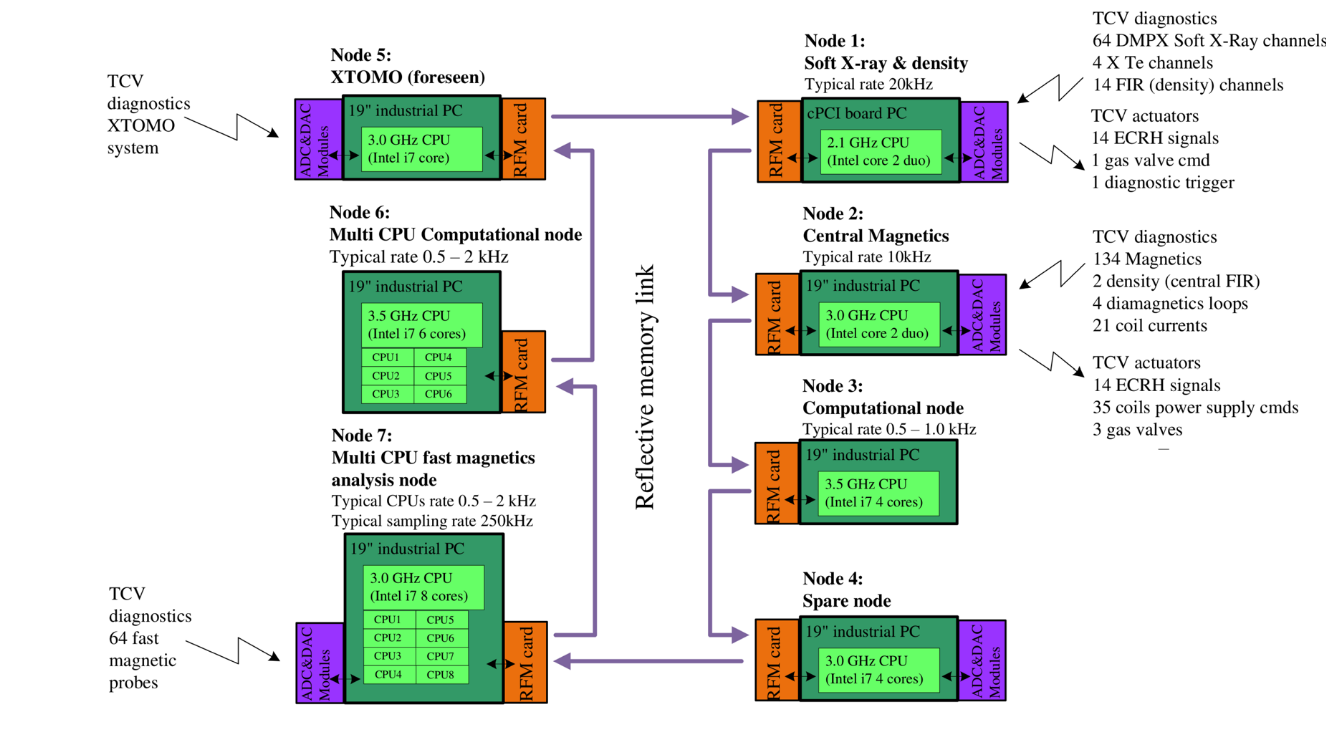
\includegraphics[width=0.65\textwidth]{Chp2/TCVcntrl1.png}
	\caption{\label{TCVcontrol} TCV SCD. Real-time network nodes connection. The nodes configurations 	are shown together with the typical diagnostic and actuator systems to which they are connected  ~\cite{TCVcntrl1}.  }
\end{figure}

\section{MARTe framework}
Regardless the nature of a real-time system the design of it is usually related to the specific requirements it has, commonly this implies to have customized hardware and software which causes a lack in modularity and portability. When systems become bigger is convenient to provide a common library containing shareable functionalities and which also allows for modular implementations. In order to deal with this the MARTe framework was designed about a decade ago. MARTe was developed in order to standardize general real-time control systems for the execution of control algorithms and is based on a multiplatform $C^{++}$ library ~\cite{Neto2010}.  Previous implementations for a  software framework similar to MARTe were developed some years before for the JET tokamak. JETRT was a software framework used to develop real-time control and data acquisition systems which laid the foundation for current MARTe framework ~\cite{JETRT}. MARTe is currently used in several tokamaks such as JET, FTU, COMPASS and ISTTOK. 

\subsection{MARTe architecture }
The unitary MARTe component is the Generic Application Module (GAM), each of the C++ programmed GAMs usually performs an specific task of the control system, the collection of interconnecting GAMs builds MARTe  \cite{Neto2011}. The GAMs  have an entry point to receive data driven configuration and a set of input and output channels to interface with other GAMs. The Dynamic Data Buffer (DDB) is a generic memory data bus where each GAM receives and produce data using DDB named channels. Usually each GAM is associated with a special function of the system like processing data of an specific diagnostic or perform some  control algorithm. MARTe hardware data interface and synchronization for inputs and outputs is performed using a special GAM called IOGAM.


\begin{figure}[htbp]
	\centering
	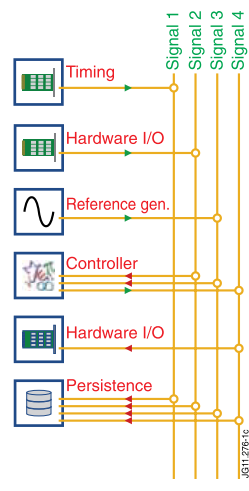
\includegraphics[width=0.35\textwidth]{Chp2/GAMs.png}
	\caption{\label{GAMs} Example of a set of GAMs connected to the DDB. Timing and hardware GAMs provide the I/O interface to the exterior, whereas a generic waveform GAM inputs the reference for a PID controller. Finally, the output is sent to a DAC and the data is stored for analysis by a collection GAM.  It should be noticed that the reference generation and the controller GAM are not aware of the changes in the data providers and data consumers.  \cite{MARTe2011}}
	
\end{figure}

\subsection{Hardware containers}

The MARTe hardware containers 


\subsection{MARTe 2.0}
Software Quality Assurance (QA)\footnote{Software QA is a set of activities or processes that define and assess the adequacy of software processes to provide evidence that establishes confidence that the software processes are appropriate for and produce software products of suitable quality for their intended purposes~\cite[Chapter 5.1]{SQA}.} processes are being applied to the development of a new version of the MARTe framework also  called MARTe 2.0. The  main objective is to provide a QA certifiable environment from where it is possible to develop, with less effort, certifiable applications. The  MARTe QA version can be easily adapted to the development of many types of software which are common in the fusion community, in particular for software related to control and data acquisition systems that is to be shared among different teams  ~\cite{MARTe2}. MARTe 2.0 will be the result of reduction exercise of the core framework based on the lessons learned from MARTe. This version will incorporate and implement an integral quality assurance process for the development of the framework (e.g. unit tests and coding standard) ~\cite{MARTe2PMP}. 
\smallskip

In order to develop robust code and to avoid common errors and pitfalls, a controlled subset of the C++ language must be defined for the MARTe framework. This subset will be define by means of a list of coding rules, which will address all dangerous aspects of the C++ language for critical systems. Thus, the C++ version used on MARTe will be defined by the standard ISO/IEC 14882:2003 aka as C++03, while the coding rules will be those defined by the standard MISRA C++:2008 ~\cite{MARTe2Code}. The MARTe project manager is responsible for appointing a quality office (QO) for the quality assurance (QA) process. The QO will guarantee that the QA activities are executed accordingly to the software development process, it will also conduct independent reviews and audit all data and processes involving the development, production and maintenance of MARTe deliverables ~\cite{MARTe2QAP}. The overall advantage of the new MARTe version is that the common faced difficulties of distributing and maintaining a software without  the continuous support of the original developers will be overcome following a complete QA system.



\section{Equilibrium and control algorithms} 

Tokamak equilibrium codes are used for retrieving information about plasma current, shape and position and pressures profiles among other parameters. Usually these codes use as input data as the machine geometry, the PF coils currents and the flux and magnetic field diagnostics measurements. The importance of these codes is that since some of the parameters necessary for an accurate feedback control are not directly measured from the diagnostics,  these data has to be fitted on real-time somehow to the Grad-Shafranov equilibrium model~\cite{Shafranov1971}. In this section some of the most implemented and reported codes for tokamak plasma equilibrium reconstruction will be briefly  described, as well as some of the most common real-time control techniques. 
\smallskip 


The EFIT (Equilibrium Fitting) code is used to efficiently reconstruct the current profile parameters, the plasma shape  and a current density profile satisfying the MHD equilibrium constraint  based on a Picard iteration\footnote{Picard iterations is a method based on  successive approximations to obtained a set of conditions under which an initial value problem has a unique solution.} approach which approximately conserves the external magnetic measurements ~\cite{EFIT1985}. EFIT has served as the de-facto standard technique to infer equilibrium from experimental diagnostics and there have been many different code implementations of this technique, all EFIT versions  are able to solve the MHD force balance and most experiment-specific customizations are made for the addition of experimental constraints peculiar to the experiment being modelled~\cite{EFIT2013}. EFIT reconstruction code is used in tokamaks such as DIII-D and the National Spherical Torus Experiment (NSTX). For the specific NSTX case they implemented a special real-time EFIT version called rtEFIT developed at General Atomics, the rtEFIT code provides the shape of the plasma boundary that is used as input to an isoflux control algorithm that generates voltage requests to the power supplies. The plasma boundaries reconstructed in real-time compare well to those reconstructed using the EFIT code offline in between plasma discharges ~\cite{rtEFIT}.
\smallskip


The RAPTOR (RApid Plasma Transport simulatOR)  is a model-based control-oriented code that predicts tokamak plasma profile evolution on real-time, it predicts the evolutions of several parameters, thanks to its accurate yet simplified physics model \cite{Raptor}. The physical model of the plant is derived from a spatially discretized partial differential equation (PDE), yielding a nonlinear set of ordinary differential equations (ODEs) for which the derivatives are evaluated analytically by the RAPTOR code. One of the main RAPTOR features is that  while the plasma is evolving RAPTOR has full knowledge of the plasma profiles and the available real-time diagnostic data can be included in a natural way to improve the accuracy of the estimation, in control engineering this approach is known as dynamic state observer and is used to estimate unmeasured or  poorly states of a dynamical system ~\cite{RAPTOR2011}. This dynamic state observer consists on an extended Kalman filter which estimates an augmented state consisting of physical states and random-walk disturbances  ~\cite{RAPTOR2014}. The concepts of  states-space systems and Kalman filtering will be addressed in the next subsections.  Figure ~\ref{RaptorMARTe} scheme shows  the carries out  integration of the RAPTOR code on top of the MARTe framework at the Italian tokamak RFX-mod.
\smallskip

For the case of JET  a  boundary reconstruction package called XLOC has been used to localized the X-point position and plasma boundary ~\cite{xloc}.  A newer code relying on XLOC  called Equinox was designed and implemented in C++ using a finite element method and a non linear fixed point algorithm associated to a least  square optimization procedure to reconstruct the plasma equilibrium in less than 50ms for the real-system~\cite{equinox}. 
\smallskip

The CREATE  codes are  equilibrium solvers that will be widely described in next chapter ~\cite{Albanese:CREATEL} and its application for the plasma control shape and  position in JT60-SA tokamak.
 
\begin{figure}[htbp]
	\centering
	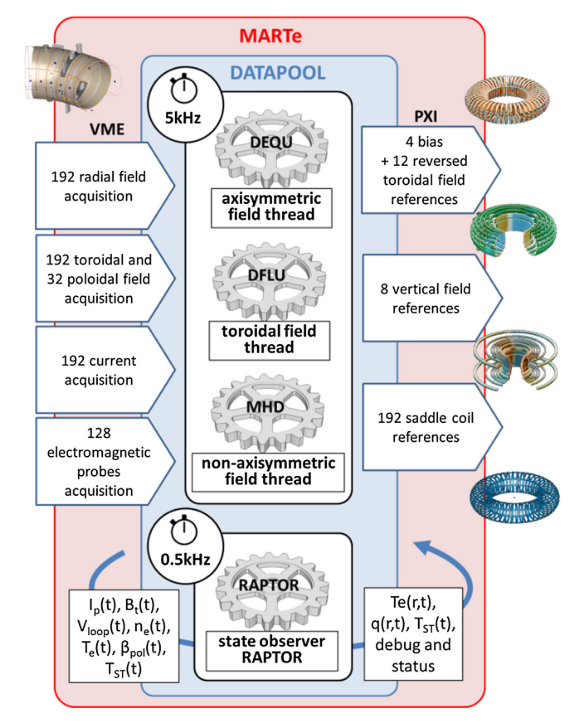
\includegraphics[width=0.505\textwidth]{Chp2/raptorMARTe.png}
	\caption{\label{RaptorMARTe} Skectch of the integration of the state observer RAPTOR in the RFX-mod real-time control system based on the MARTe framework.
		experimental \cite{Raptor}}
	
\end{figure}




\subsection{State-Space models}

State-space models will be crucial for the overall development of the work presented on this thesis whether they will be use to describe a tokamak linear model for plasma position and  shape control or use to model some other relevant variables. This section will summarize  some systems dynamics and control  concepts which will be applied on the next chapters. The first concepts  to be summarized on this section are the state variable and state equation definitions.   \smallskip

Let the $n$ state equations of $nth$-order dynamic system be represented as:

\begin{equation}
	\frac{dx_1 (t)}{dt} ~ = ~ f_i [x_1(t),x_2(t),...,x_n(t), u_1(t),u_2(t),...,u_p(t),w_1(t)w_2(t),...,w_v(t)]
	\label{stateEqs}
\end{equation}

 where $i=1,2,..,n$. The $ith$ state variable is represented by $x_i(t)$; $u_j(t)$ denotes the $jth$ input for $j=1,2,..,p$; and $w_k(t)$ denotes the $kth$ disturbance input, with $k=1,2,..,v~$.\smallskip
 
 Let $y_1(t),y_2(t),...,y_q(t) $ be the q system output variables. The output variables are functions of the state variables  and the input variables. The output equations can be expressed as:
 \begin{equation}
 	y_j(t)=g_j[x_1(t),x_2(t),...,x_n(t),u_1(t),u_2(t),..,u_p(t),w_1(t)w_2(t),...,w_v(t)]
 \label{outputEq}
 \end{equation}
 
 where $j=1,2,..,q$~.
 \smallskip
 
 The set of $n$ state equations from ~\ref{stateEqs} and the $q$ output equations in ~\ref{outputEq} together they form the \textit{dynamic equations}. In order to have an easier form of expression and manipulations of these equations is common to represent them in vectors and matrices as follows: \smallskip
 \begin{equation}
 x(t)=
 \left[
 	\begin{matrix}
 	x_1(t)\\
 	x_2(t)\\
 	\vdots\\
 	x_n(t)
 	\end{matrix}
 	\right] \, (n\times 1)
 \end{equation}
 
 
  \begin{equation}
 u(t)=
 \left[
 \begin{matrix}
 u_1(t)\\
 u_2(t)\\
 \vdots\\
 u_p(t)
 \end{matrix}
 \right] \, (p\times 1)
 \end{equation}
 
   \begin{equation}
y(t)=
 \left[
 \begin{matrix}
 y_1(t)\\
 y_2(t)\\
 \vdots\\
 y_q(t)
 \end{matrix}
 \right] \, (q\times 1)
 \end{equation}
 
    \begin{equation}
 w(t)=
 \left[
 \begin{matrix}
 w_1(t)\\
 w_2(t)\\
 \vdots\\
 w_v(t)
 \end{matrix}
 \right] \, (v\times 1)
 \end{equation}
 
 Using these defined vectors, equation ~\ref{stateEqs} can be write for the $n$ states like:\smallskip
 
 \begin{equation}
 	\frac{dx(t)}{dt}~=~ f[x(t),u(t),w(t)]
 \end{equation} 
 where f is a vector containing the functions $f_1,f_2,..,f_n$ as elements. In the same way the equations from ~\ref{outputEq} become:
 \begin{equation}
 	y(t)=g[x(t),u(t),w(t)]
 \end{equation}
 where $g$ is a vector containing the functions $g_1,g_2,..,g_n$ as elements.
 
 For a system that is time-invariant and linear like the ones that will show on next chapter, the equations can be re-write as:
 
 \begin{equation}
 	\frac{dx(t)}{dt}~=~ Ax(t)~+~Bu(t)~+E_(w)
 \end{equation}
 
 \begin{equation}
y(t)=Cx(t)+Du(t)+Hw(t)
 \end{equation}
  where $A,B,C,D, E and H$ are matrices.
 
\subsection{PID control}

Proportional-Integral-Derivative (PID) control 

\subsection{Multiple-Input Multiple-Output control}

Multiple-Input Multiple-Output (MIMO)

\subsection{Kalman filtering}

